\documentclass[a4paper,fleqn]{cas-sc}
\usepackage[numbers]{natbib}
\usepackage{amsmath,amssymb,amsthm,booktabs,graphicx}
\usepackage{placeins}
\newtheorem{proposition}{Proposition}
\newcommand{\AMO}{\mathrm{AMO}}
\newcommand{\ALO}{\mathrm{ALO}}
\newcommand{\EO}{\mathrm{EO}}
% Generated by nqueens.analyze and nqueens.report_details; do not edit.
\makeatletter
\providecommand{\res}[1]{\ifcsname res@#1\endcsname\csname res@#1\endcsname\else\PackageError{numbers}{Unknown result key #1}{}\fi}
\@namedef{res@all/cadical195-commander-minimal/par2}{55.71}
\@namedef{res@all/cadical195-commander-minimal/solved}{7/8}
\@namedef{res@all/cplex-cp/par2}{4.26}
\@namedef{res@all/cplex-cp/solved}{8/8}
\@namedef{res@all/cplex-mip/par2}{47.61}
\@namedef{res@all/cplex-mip/solved}{7/8}
\@namedef{res@all/cpsat/par2}{102.1}
\@namedef{res@all/cpsat/solved}{6/8}
\@namedef{res@all/gurobi/par2}{3.82}
\@namedef{res@all/gurobi/solved}{8/8}
\@namedef{res@budget}{180}
\@namedef{res@checked}{110}
\@namedef{res@cost/binary-extended/build}{3.18}
\@namedef{res@cost/binary-extended/solve}{11.63}
\@namedef{res@cost/binary-minimal/build}{3.03}
\@namedef{res@cost/binary-minimal/solve}{71.29}
\@namedef{res@cost/commander-extended/build}{2.90}
\@namedef{res@cost/commander-extended/solve}{4.57}
\@namedef{res@cost/commander-minimal/build}{1.34}
\@namedef{res@cost/commander-minimal/solve}{2.72}
\@namedef{res@cost/product-extended/build}{1.87}
\@namedef{res@cost/product-extended/solve}{15.35}
\@namedef{res@cost/seqcounter-extended/build}{2.78}
\@namedef{res@cost/seqcounter-extended/solve}{122.6}
\@namedef{res@encodings/best}{commander/minimal}
\@namedef{res@encodings/cadical195-binary-extended/128/core}{6.44}
\@namedef{res@encodings/cadical195-binary-extended/128/solved}{1/1}
\@namedef{res@encodings/cadical195-binary-extended/128/time}{6.80}
\@namedef{res@encodings/cadical195-binary-extended/16/core}{0.05}
\@namedef{res@encodings/cadical195-binary-extended/16/solved}{1/1}
\@namedef{res@encodings/cadical195-binary-extended/16/time}{0.50}
\@namedef{res@encodings/cadical195-binary-extended/256/core}{14.81}
\@namedef{res@encodings/cadical195-binary-extended/256/solved}{1/1}
\@namedef{res@encodings/cadical195-binary-extended/256/time}{15.16}
\@namedef{res@encodings/cadical195-binary-extended/32/core}{0.29}
\@namedef{res@encodings/cadical195-binary-extended/32/solved}{1/1}
\@namedef{res@encodings/cadical195-binary-extended/32/time}{0.74}
\@namedef{res@encodings/cadical195-binary-extended/64/core}{0.81}
\@namedef{res@encodings/cadical195-binary-extended/64/solved}{1/1}
\@namedef{res@encodings/cadical195-binary-extended/64/time}{1.19}
\@namedef{res@encodings/cadical195-binary-extended/8/core}{0.00}
\@namedef{res@encodings/cadical195-binary-extended/8/solved}{1/1}
\@namedef{res@encodings/cadical195-binary-extended/8/time}{0.48}
\@namedef{res@encodings/cadical195-binary-extended/clauses}{2,053,460}
\@namedef{res@encodings/cadical195-binary-extended/par2}{4.15}
\@namedef{res@encodings/cadical195-binary-extended/solved}{6/6}
\@namedef{res@encodings/cadical195-binary-extended/vars}{76,784}
\@namedef{res@encodings/cadical195-binary-minimal/128/core}{15.84}
\@namedef{res@encodings/cadical195-binary-minimal/128/solved}{1/1}
\@namedef{res@encodings/cadical195-binary-minimal/128/time}{16.35}
\@namedef{res@encodings/cadical195-binary-minimal/16/core}{0.03}
\@namedef{res@encodings/cadical195-binary-minimal/16/solved}{1/1}
\@namedef{res@encodings/cadical195-binary-minimal/16/time}{0.57}
\@namedef{res@encodings/cadical195-binary-minimal/256/core}{74.32}
\@namedef{res@encodings/cadical195-binary-minimal/256/solved}{1/1}
\@namedef{res@encodings/cadical195-binary-minimal/256/time}{74.71}
\@namedef{res@encodings/cadical195-binary-minimal/32/core}{0.23}
\@namedef{res@encodings/cadical195-binary-minimal/32/solved}{1/1}
\@namedef{res@encodings/cadical195-binary-minimal/32/time}{0.67}
\@namedef{res@encodings/cadical195-binary-minimal/64/core}{4.61}
\@namedef{res@encodings/cadical195-binary-minimal/64/solved}{1/1}
\@namedef{res@encodings/cadical195-binary-minimal/64/time}{5.04}
\@namedef{res@encodings/cadical195-binary-minimal/8/core}{0.01}
\@namedef{res@encodings/cadical195-binary-minimal/8/solved}{1/1}
\@namedef{res@encodings/cadical195-binary-minimal/8/time}{0.66}
\@namedef{res@encodings/cadical195-binary-minimal/clauses}{2,053,204}
\@namedef{res@encodings/cadical195-binary-minimal/par2}{16.33}
\@namedef{res@encodings/cadical195-binary-minimal/solved}{6/6}
\@namedef{res@encodings/cadical195-binary-minimal/vars}{76,784}
\@namedef{res@encodings/cadical195-commander-extended/128/core}{0.92}
\@namedef{res@encodings/cadical195-commander-extended/128/solved}{1/1}
\@namedef{res@encodings/cadical195-commander-extended/128/time}{1.32}
\@namedef{res@encodings/cadical195-commander-extended/16/core}{0.01}
\@namedef{res@encodings/cadical195-commander-extended/16/solved}{1/1}
\@namedef{res@encodings/cadical195-commander-extended/16/time}{0.50}
\@namedef{res@encodings/cadical195-commander-extended/256/core}{7.47}
\@namedef{res@encodings/cadical195-commander-extended/256/solved}{1/1}
\@namedef{res@encodings/cadical195-commander-extended/256/time}{8.17}
\@namedef{res@encodings/cadical195-commander-extended/32/core}{0.04}
\@namedef{res@encodings/cadical195-commander-extended/32/solved}{1/1}
\@namedef{res@encodings/cadical195-commander-extended/32/time}{0.57}
\@namedef{res@encodings/cadical195-commander-extended/64/core}{0.18}
\@namedef{res@encodings/cadical195-commander-extended/64/solved}{1/1}
\@namedef{res@encodings/cadical195-commander-extended/64/time}{0.60}
\@namedef{res@encodings/cadical195-commander-extended/8/core}{0.00}
\@namedef{res@encodings/cadical195-commander-extended/8/solved}{1/1}
\@namedef{res@encodings/cadical195-commander-extended/8/time}{0.53}
\@namedef{res@encodings/cadical195-commander-extended/clauses}{912,010}
\@namedef{res@encodings/cadical195-commander-extended/par2}{1.95}
\@namedef{res@encodings/cadical195-commander-extended/solved}{6/6}
\@namedef{res@encodings/cadical195-commander-extended/vars}{197,342}
\@namedef{res@encodings/cadical195-commander-minimal/128/core}{0.96}
\@namedef{res@encodings/cadical195-commander-minimal/128/solved}{1/1}
\@namedef{res@encodings/cadical195-commander-minimal/128/time}{1.36}
\@namedef{res@encodings/cadical195-commander-minimal/16/core}{0.01}
\@namedef{res@encodings/cadical195-commander-minimal/16/solved}{1/1}
\@namedef{res@encodings/cadical195-commander-minimal/16/time}{0.59}
\@namedef{res@encodings/cadical195-commander-minimal/256/core}{4.06}
\@namedef{res@encodings/cadical195-commander-minimal/256/solved}{1/1}
\@namedef{res@encodings/cadical195-commander-minimal/256/time}{4.51}
\@namedef{res@encodings/cadical195-commander-minimal/32/core}{0.06}
\@namedef{res@encodings/cadical195-commander-minimal/32/solved}{1/1}
\@namedef{res@encodings/cadical195-commander-minimal/32/time}{0.60}
\@namedef{res@encodings/cadical195-commander-minimal/64/core}{0.20}
\@namedef{res@encodings/cadical195-commander-minimal/64/solved}{1/1}
\@namedef{res@encodings/cadical195-commander-minimal/64/time}{0.62}
\@namedef{res@encodings/cadical195-commander-minimal/8/core}{0.00}
\@namedef{res@encodings/cadical195-commander-minimal/8/solved}{1/1}
\@namedef{res@encodings/cadical195-commander-minimal/8/time}{0.57}
\@namedef{res@encodings/cadical195-commander-minimal/clauses}{911,754}
\@namedef{res@encodings/cadical195-commander-minimal/par2}{1.38}
\@namedef{res@encodings/cadical195-commander-minimal/solved}{6/6}
\@namedef{res@encodings/cadical195-commander-minimal/vars}{197,342}
\@namedef{res@encodings/cadical195-pairwise-extended/128/core}{9.60}
\@namedef{res@encodings/cadical195-pairwise-extended/128/solved}{1/1}
\@namedef{res@encodings/cadical195-pairwise-extended/128/time}{9.95}
\@namedef{res@encodings/cadical195-pairwise-extended/16/core}{0.02}
\@namedef{res@encodings/cadical195-pairwise-extended/16/solved}{1/1}
\@namedef{res@encodings/cadical195-pairwise-extended/16/time}{0.52}
\@namedef{res@encodings/cadical195-pairwise-extended/256/core}{TO}
\@namedef{res@encodings/cadical195-pairwise-extended/256/solved}{0/1}
\@namedef{res@encodings/cadical195-pairwise-extended/256/time}{TO}
\@namedef{res@encodings/cadical195-pairwise-extended/32/core}{0.39}
\@namedef{res@encodings/cadical195-pairwise-extended/32/solved}{1/1}
\@namedef{res@encodings/cadical195-pairwise-extended/32/time}{0.86}
\@namedef{res@encodings/cadical195-pairwise-extended/64/core}{1.08}
\@namedef{res@encodings/cadical195-pairwise-extended/64/solved}{1/1}
\@namedef{res@encodings/cadical195-pairwise-extended/64/time}{1.43}
\@namedef{res@encodings/cadical195-pairwise-extended/8/core}{0.00}
\@namedef{res@encodings/cadical195-pairwise-extended/8/solved}{1/1}
\@namedef{res@encodings/cadical195-pairwise-extended/8/time}{0.48}
\@namedef{res@encodings/cadical195-pairwise-extended/clauses}{27,831,552}
\@namedef{res@encodings/cadical195-pairwise-extended/par2}{62.21}
\@namedef{res@encodings/cadical195-pairwise-extended/solved}{5/6}
\@namedef{res@encodings/cadical195-pairwise-extended/vars}{65,536}
\@namedef{res@encodings/cadical195-pairwise-minimal/128/core}{7.59}
\@namedef{res@encodings/cadical195-pairwise-minimal/128/solved}{1/1}
\@namedef{res@encodings/cadical195-pairwise-minimal/128/time}{8.06}
\@namedef{res@encodings/cadical195-pairwise-minimal/16/core}{0.02}
\@namedef{res@encodings/cadical195-pairwise-minimal/16/solved}{1/1}
\@namedef{res@encodings/cadical195-pairwise-minimal/16/time}{0.56}
\@namedef{res@encodings/cadical195-pairwise-minimal/256/core}{TO}
\@namedef{res@encodings/cadical195-pairwise-minimal/256/solved}{0/1}
\@namedef{res@encodings/cadical195-pairwise-minimal/256/time}{TO}
\@namedef{res@encodings/cadical195-pairwise-minimal/32/core}{0.24}
\@namedef{res@encodings/cadical195-pairwise-minimal/32/solved}{1/1}
\@namedef{res@encodings/cadical195-pairwise-minimal/32/time}{0.76}
\@namedef{res@encodings/cadical195-pairwise-minimal/64/core}{2.03}
\@namedef{res@encodings/cadical195-pairwise-minimal/64/solved}{1/1}
\@namedef{res@encodings/cadical195-pairwise-minimal/64/time}{2.44}
\@namedef{res@encodings/cadical195-pairwise-minimal/8/core}{0.00}
\@namedef{res@encodings/cadical195-pairwise-minimal/8/solved}{1/1}
\@namedef{res@encodings/cadical195-pairwise-minimal/8/time}{0.46}
\@namedef{res@encodings/cadical195-pairwise-minimal/clauses}{27,831,296}
\@namedef{res@encodings/cadical195-pairwise-minimal/par2}{62.05}
\@namedef{res@encodings/cadical195-pairwise-minimal/solved}{5/6}
\@namedef{res@encodings/cadical195-pairwise-minimal/vars}{65,536}
\@namedef{res@encodings/cadical195-product-extended/128/core}{5.60}
\@namedef{res@encodings/cadical195-product-extended/128/solved}{1/1}
\@namedef{res@encodings/cadical195-product-extended/128/time}{5.94}
\@namedef{res@encodings/cadical195-product-extended/16/core}{0.02}
\@namedef{res@encodings/cadical195-product-extended/16/solved}{1/1}
\@namedef{res@encodings/cadical195-product-extended/16/time}{0.53}
\@namedef{res@encodings/cadical195-product-extended/256/core}{17.22}
\@namedef{res@encodings/cadical195-product-extended/256/solved}{1/1}
\@namedef{res@encodings/cadical195-product-extended/256/time}{17.73}
\@namedef{res@encodings/cadical195-product-extended/32/core}{0.76}
\@namedef{res@encodings/cadical195-product-extended/32/solved}{1/1}
\@namedef{res@encodings/cadical195-product-extended/32/time}{1.23}
\@namedef{res@encodings/cadical195-product-extended/64/core}{0.93}
\@namedef{res@encodings/cadical195-product-extended/64/solved}{1/1}
\@namedef{res@encodings/cadical195-product-extended/64/time}{1.27}
\@namedef{res@encodings/cadical195-product-extended/8/core}{0.00}
\@namedef{res@encodings/cadical195-product-extended/8/solved}{1/1}
\@namedef{res@encodings/cadical195-product-extended/8/time}{0.46}
\@namedef{res@encodings/cadical195-product-extended/clauses}{631,720}
\@namedef{res@encodings/cadical195-product-extended/par2}{4.53}
\@namedef{res@encodings/cadical195-product-extended/solved}{6/6}
\@namedef{res@encodings/cadical195-product-extended/vars}{125,800}
\@namedef{res@encodings/cadical195-product-minimal/128/core}{TO}
\@namedef{res@encodings/cadical195-product-minimal/128/solved}{0/1}
\@namedef{res@encodings/cadical195-product-minimal/128/time}{TO}
\@namedef{res@encodings/cadical195-product-minimal/16/core}{0.03}
\@namedef{res@encodings/cadical195-product-minimal/16/solved}{1/1}
\@namedef{res@encodings/cadical195-product-minimal/16/time}{0.52}
\@namedef{res@encodings/cadical195-product-minimal/256/core}{TO}
\@namedef{res@encodings/cadical195-product-minimal/256/solved}{0/1}
\@namedef{res@encodings/cadical195-product-minimal/256/time}{TO}
\@namedef{res@encodings/cadical195-product-minimal/32/core}{1.29}
\@namedef{res@encodings/cadical195-product-minimal/32/solved}{1/1}
\@namedef{res@encodings/cadical195-product-minimal/32/time}{1.75}
\@namedef{res@encodings/cadical195-product-minimal/64/core}{13.43}
\@namedef{res@encodings/cadical195-product-minimal/64/solved}{1/1}
\@namedef{res@encodings/cadical195-product-minimal/64/time}{13.86}
\@namedef{res@encodings/cadical195-product-minimal/8/core}{0.01}
\@namedef{res@encodings/cadical195-product-minimal/8/solved}{1/1}
\@namedef{res@encodings/cadical195-product-minimal/8/time}{0.57}
\@namedef{res@encodings/cadical195-product-minimal/clauses}{631,464}
\@namedef{res@encodings/cadical195-product-minimal/par2}{122.8}
\@namedef{res@encodings/cadical195-product-minimal/solved}{4/6}
\@namedef{res@encodings/cadical195-product-minimal/vars}{125,800}
\@namedef{res@encodings/cadical195-seqcounter-extended/128/core}{6.98}
\@namedef{res@encodings/cadical195-seqcounter-extended/128/solved}{1/1}
\@namedef{res@encodings/cadical195-seqcounter-extended/128/time}{7.42}
\@namedef{res@encodings/cadical195-seqcounter-extended/16/core}{0.05}
\@namedef{res@encodings/cadical195-seqcounter-extended/16/solved}{1/1}
\@namedef{res@encodings/cadical195-seqcounter-extended/16/time}{0.50}
\@namedef{res@encodings/cadical195-seqcounter-extended/256/core}{125.4}
\@namedef{res@encodings/cadical195-seqcounter-extended/256/solved}{1/1}
\@namedef{res@encodings/cadical195-seqcounter-extended/256/time}{126.0}
\@namedef{res@encodings/cadical195-seqcounter-extended/32/core}{0.16}
\@namedef{res@encodings/cadical195-seqcounter-extended/32/solved}{1/1}
\@namedef{res@encodings/cadical195-seqcounter-extended/32/time}{0.59}
\@namedef{res@encodings/cadical195-seqcounter-extended/64/core}{2.07}
\@namedef{res@encodings/cadical195-seqcounter-extended/64/solved}{1/1}
\@namedef{res@encodings/cadical195-seqcounter-extended/64/time}{2.43}
\@namedef{res@encodings/cadical195-seqcounter-extended/8/core}{0.00}
\@namedef{res@encodings/cadical195-seqcounter-extended/8/solved}{1/1}
\@namedef{res@encodings/cadical195-seqcounter-extended/8/time}{0.53}
\@namedef{res@encodings/cadical195-seqcounter-extended/clauses}{780,808}
\@namedef{res@encodings/cadical195-seqcounter-extended/par2}{22.92}
\@namedef{res@encodings/cadical195-seqcounter-extended/solved}{6/6}
\@namedef{res@encodings/cadical195-seqcounter-extended/vars}{326,142}
\@namedef{res@encodings/cadical195-seqcounter-minimal/128/core}{56.65}
\@namedef{res@encodings/cadical195-seqcounter-minimal/128/solved}{1/1}
\@namedef{res@encodings/cadical195-seqcounter-minimal/128/time}{57.08}
\@namedef{res@encodings/cadical195-seqcounter-minimal/16/core}{0.01}
\@namedef{res@encodings/cadical195-seqcounter-minimal/16/solved}{1/1}
\@namedef{res@encodings/cadical195-seqcounter-minimal/16/time}{0.44}
\@namedef{res@encodings/cadical195-seqcounter-minimal/256/core}{TO}
\@namedef{res@encodings/cadical195-seqcounter-minimal/256/solved}{0/1}
\@namedef{res@encodings/cadical195-seqcounter-minimal/256/time}{TO}
\@namedef{res@encodings/cadical195-seqcounter-minimal/32/core}{0.21}
\@namedef{res@encodings/cadical195-seqcounter-minimal/32/solved}{1/1}
\@namedef{res@encodings/cadical195-seqcounter-minimal/32/time}{0.65}
\@namedef{res@encodings/cadical195-seqcounter-minimal/64/core}{12.01}
\@namedef{res@encodings/cadical195-seqcounter-minimal/64/solved}{1/1}
\@namedef{res@encodings/cadical195-seqcounter-minimal/64/time}{12.38}
\@namedef{res@encodings/cadical195-seqcounter-minimal/8/core}{0.00}
\@namedef{res@encodings/cadical195-seqcounter-minimal/8/solved}{1/1}
\@namedef{res@encodings/cadical195-seqcounter-minimal/8/time}{0.55}
\@namedef{res@encodings/cadical195-seqcounter-minimal/clauses}{780,552}
\@namedef{res@encodings/cadical195-seqcounter-minimal/par2}{71.85}
\@namedef{res@encodings/cadical195-seqcounter-minimal/solved}{5/6}
\@namedef{res@encodings/cadical195-seqcounter-minimal/vars}{326,142}
\@namedef{res@encodings/maxn}{256}
\@namedef{res@errors}{0}
\@namedef{res@exact/cadical195-commander-minimal/128/core}{1.17}
\@namedef{res@exact/cadical195-commander-minimal/128/solved}{1/1}
\@namedef{res@exact/cadical195-commander-minimal/128/time}{1.61}
\@namedef{res@exact/cadical195-commander-minimal/16/core}{0.01}
\@namedef{res@exact/cadical195-commander-minimal/16/solved}{1/1}
\@namedef{res@exact/cadical195-commander-minimal/16/time}{0.58}
\@namedef{res@exact/cadical195-commander-minimal/256/core}{8.97}
\@namedef{res@exact/cadical195-commander-minimal/256/solved}{1/1}
\@namedef{res@exact/cadical195-commander-minimal/256/time}{10.03}
\@namedef{res@exact/cadical195-commander-minimal/32/core}{0.05}
\@namedef{res@exact/cadical195-commander-minimal/32/solved}{1/1}
\@namedef{res@exact/cadical195-commander-minimal/32/time}{0.62}
\@namedef{res@exact/cadical195-commander-minimal/64/core}{0.22}
\@namedef{res@exact/cadical195-commander-minimal/64/solved}{1/1}
\@namedef{res@exact/cadical195-commander-minimal/64/time}{0.76}
\@namedef{res@exact/cadical195-commander-minimal/8/core}{0.01}
\@namedef{res@exact/cadical195-commander-minimal/8/solved}{1/1}
\@namedef{res@exact/cadical195-commander-minimal/8/time}{0.63}
\@namedef{res@exact/cadical195-commander-minimal/par2}{2.37}
\@namedef{res@exact/cadical195-commander-minimal/solved}{6/6}
\@namedef{res@exact/cplex-cp/128/core}{0.07}
\@namedef{res@exact/cplex-cp/128/solved}{1/1}
\@namedef{res@exact/cplex-cp/128/time}{2.52}
\@namedef{res@exact/cplex-cp/16/core}{0.06}
\@namedef{res@exact/cplex-cp/16/solved}{1/1}
\@namedef{res@exact/cplex-cp/16/time}{3.06}
\@namedef{res@exact/cplex-cp/256/core}{0.10}
\@namedef{res@exact/cplex-cp/256/solved}{1/1}
\@namedef{res@exact/cplex-cp/256/time}{3.20}
\@namedef{res@exact/cplex-cp/32/core}{0.08}
\@namedef{res@exact/cplex-cp/32/solved}{1/1}
\@namedef{res@exact/cplex-cp/32/time}{3.07}
\@namedef{res@exact/cplex-cp/64/core}{0.07}
\@namedef{res@exact/cplex-cp/64/solved}{1/1}
\@namedef{res@exact/cplex-cp/64/time}{3.11}
\@namedef{res@exact/cplex-cp/8/core}{0.07}
\@namedef{res@exact/cplex-cp/8/solved}{1/1}
\@namedef{res@exact/cplex-cp/8/time}{3.19}
\@namedef{res@exact/cplex-cp/par2}{3.02}
\@namedef{res@exact/cplex-cp/solved}{6/6}
\@namedef{res@exact/cplex-mip/128/core}{0.41}
\@namedef{res@exact/cplex-mip/128/solved}{1/1}
\@namedef{res@exact/cplex-mip/128/time}{1.09}
\@namedef{res@exact/cplex-mip/16/core}{0.02}
\@namedef{res@exact/cplex-mip/16/solved}{1/1}
\@namedef{res@exact/cplex-mip/16/time}{0.74}
\@namedef{res@exact/cplex-mip/256/core}{3.13}
\@namedef{res@exact/cplex-mip/256/solved}{1/1}
\@namedef{res@exact/cplex-mip/256/time}{3.92}
\@namedef{res@exact/cplex-mip/32/core}{0.02}
\@namedef{res@exact/cplex-mip/32/solved}{1/1}
\@namedef{res@exact/cplex-mip/32/time}{0.79}
\@namedef{res@exact/cplex-mip/64/core}{0.08}
\@namedef{res@exact/cplex-mip/64/solved}{1/1}
\@namedef{res@exact/cplex-mip/64/time}{0.90}
\@namedef{res@exact/cplex-mip/8/core}{0.03}
\@namedef{res@exact/cplex-mip/8/solved}{1/1}
\@namedef{res@exact/cplex-mip/8/time}{0.76}
\@namedef{res@exact/cplex-mip/par2}{1.37}
\@namedef{res@exact/cplex-mip/solved}{6/6}
\@namedef{res@exact/cpsat/128/core}{5.92}
\@namedef{res@exact/cpsat/128/solved}{1/1}
\@namedef{res@exact/cpsat/128/time}{8.36}
\@namedef{res@exact/cpsat/16/core}{0.04}
\@namedef{res@exact/cpsat/16/solved}{1/1}
\@namedef{res@exact/cpsat/16/time}{2.78}
\@namedef{res@exact/cpsat/256/core}{44.63}
\@namedef{res@exact/cpsat/256/solved}{1/1}
\@namedef{res@exact/cpsat/256/time}{77.52}
\@namedef{res@exact/cpsat/32/core}{0.13}
\@namedef{res@exact/cpsat/32/solved}{1/1}
\@namedef{res@exact/cpsat/32/time}{2.85}
\@namedef{res@exact/cpsat/64/core}{0.72}
\@namedef{res@exact/cpsat/64/solved}{1/1}
\@namedef{res@exact/cpsat/64/time}{2.97}
\@namedef{res@exact/cpsat/8/core}{0.02}
\@namedef{res@exact/cpsat/8/solved}{1/1}
\@namedef{res@exact/cpsat/8/time}{2.65}
\@namedef{res@exact/cpsat/par2}{16.19}
\@namedef{res@exact/cpsat/solved}{6/6}
\@namedef{res@exact/gurobi/128/core}{0.63}
\@namedef{res@exact/gurobi/128/solved}{1/1}
\@namedef{res@exact/gurobi/128/time}{1.22}
\@namedef{res@exact/gurobi/16/core}{0.01}
\@namedef{res@exact/gurobi/16/solved}{1/1}
\@namedef{res@exact/gurobi/16/time}{0.65}
\@namedef{res@exact/gurobi/256/core}{0.72}
\@namedef{res@exact/gurobi/256/solved}{1/1}
\@namedef{res@exact/gurobi/256/time}{1.62}
\@namedef{res@exact/gurobi/32/core}{0.01}
\@namedef{res@exact/gurobi/32/solved}{1/1}
\@namedef{res@exact/gurobi/32/time}{0.70}
\@namedef{res@exact/gurobi/64/core}{0.12}
\@namedef{res@exact/gurobi/64/solved}{1/1}
\@namedef{res@exact/gurobi/64/time}{0.66}
\@namedef{res@exact/gurobi/8/core}{0.01}
\@namedef{res@exact/gurobi/8/solved}{1/1}
\@namedef{res@exact/gurobi/8/time}{0.75}
\@namedef{res@exact/gurobi/par2}{0.93}
\@namedef{res@exact/gurobi/solved}{6/6}
\@namedef{res@exact/maxn}{1024}
\@namedef{res@exact/runs}{8}
\@namedef{res@par2penalty}{360}
\@namedef{res@runs}{124}
\@namedef{res@scaling/cadical195-commander-minimal/1024/core}{TO}
\@namedef{res@scaling/cadical195-commander-minimal/1024/solved}{0/1}
\@namedef{res@scaling/cadical195-commander-minimal/1024/time}{TO}
\@namedef{res@scaling/cadical195-commander-minimal/512/core}{68.31}
\@namedef{res@scaling/cadical195-commander-minimal/512/solved}{1/1}
\@namedef{res@scaling/cadical195-commander-minimal/512/time}{71.47}
\@namedef{res@scaling/cadical195-commander-minimal/par2}{215.7}
\@namedef{res@scaling/cadical195-commander-minimal/solved}{1/2}
\@namedef{res@scaling/cplex-cp/1024/core}{1.46}
\@namedef{res@scaling/cplex-cp/1024/solved}{1/1}
\@namedef{res@scaling/cplex-cp/1024/time}{10.21}
\@namedef{res@scaling/cplex-cp/512/core}{0.22}
\@namedef{res@scaling/cplex-cp/512/solved}{1/1}
\@namedef{res@scaling/cplex-cp/512/time}{5.77}
\@namedef{res@scaling/cplex-cp/par2}{7.99}
\@namedef{res@scaling/cplex-cp/solved}{2/2}
\@namedef{res@scaling/cplex-mip/1024/core}{TO}
\@namedef{res@scaling/cplex-mip/1024/solved}{0/1}
\@namedef{res@scaling/cplex-mip/1024/time}{TO}
\@namedef{res@scaling/cplex-mip/512/core}{11.58}
\@namedef{res@scaling/cplex-mip/512/solved}{1/1}
\@namedef{res@scaling/cplex-mip/512/time}{12.65}
\@namedef{res@scaling/cplex-mip/par2}{186.3}
\@namedef{res@scaling/cplex-mip/solved}{1/2}
\@namedef{res@scaling/cpsat/1024/core}{TO}
\@namedef{res@scaling/cpsat/1024/solved}{0/1}
\@namedef{res@scaling/cpsat/1024/time}{TO}
\@namedef{res@scaling/cpsat/512/core}{TO}
\@namedef{res@scaling/cpsat/512/solved}{0/1}
\@namedef{res@scaling/cpsat/512/time}{TO}
\@namedef{res@scaling/cpsat/par2}{360.0}
\@namedef{res@scaling/cpsat/solved}{0/2}
\@namedef{res@scaling/gurobi/1024/core}{14.50}
\@namedef{res@scaling/gurobi/1024/solved}{1/1}
\@namedef{res@scaling/gurobi/1024/time}{19.76}
\@namedef{res@scaling/gurobi/512/core}{3.00}
\@namedef{res@scaling/gurobi/512/solved}{1/1}
\@namedef{res@scaling/gurobi/512/time}{5.21}
\@namedef{res@scaling/gurobi/par2}{12.48}
\@namedef{res@scaling/gurobi/solved}{2/2}
\@namedef{res@size/binary/128/clauses}{447,700}
\@namedef{res@size/binary/128/vars}{21,234}
\@namedef{res@size/binary/16/clauses}{3,908}
\@namedef{res@size/binary/16/vars}{568}
\@namedef{res@size/binary/256/clauses}{2,053,204}
\@namedef{res@size/binary/256/vars}{76,784}
\@namedef{res@size/binary/32/clauses}{19,764}
\@namedef{res@size/binary/32/vars}{1,846}
\@namedef{res@size/binary/64/clauses}{95,508}
\@namedef{res@size/binary/64/vars}{6,132}
\@namedef{res@size/binary/8/clauses}{716}
\@namedef{res@size/binary/8/vars}{170}
\@namedef{res@size/commander/128/clauses}{226,242}
\@namedef{res@size/commander/128/vars}{49,354}
\@namedef{res@size/commander/16/clauses}{3,096}
\@namedef{res@size/commander/16/vars}{712}
\@namedef{res@size/commander/256/clauses}{911,754}
\@namedef{res@size/commander/256/vars}{197,342}
\@namedef{res@size/commander/32/clauses}{13,182}
\@namedef{res@size/commander/32/vars}{2,918}
\@namedef{res@size/commander/64/clauses}{55,718}
\@namedef{res@size/commander/64/vars}{12,338}
\@namedef{res@size/commander/8/clauses}{610}
\@namedef{res@size/commander/8/vars}{146}
\@namedef{res@size/pairwise/128/clauses}{3,462,656}
\@namedef{res@size/pairwise/128/vars}{16,384}
\@namedef{res@size/pairwise/16/clauses}{6,336}
\@namedef{res@size/pairwise/16/vars}{256}
\@namedef{res@size/pairwise/256/clauses}{27,831,296}
\@namedef{res@size/pairwise/256/vars}{65,536}
\@namedef{res@size/pairwise/32/clauses}{52,608}
\@namedef{res@size/pairwise/32/vars}{1,024}
\@namedef{res@size/pairwise/64/clauses}{428,800}
\@namedef{res@size/pairwise/64/vars}{4,096}
\@namedef{res@size/pairwise/8/clauses}{736}
\@namedef{res@size/pairwise/8/vars}{64}
\@namedef{res@size/product/128/clauses}{168,984}
\@namedef{res@size/product/128/vars}{39,174}
\@namedef{res@size/product/16/clauses}{2,788}
\@namedef{res@size/product/16/vars}{820}
\@namedef{res@size/product/256/clauses}{631,464}
\@namedef{res@size/product/256/vars}{125,800}
\@namedef{res@size/product/32/clauses}{12,308}
\@namedef{res@size/product/32/vars}{3,932}
\@namedef{res@size/product/64/clauses}{45,556}
\@namedef{res@size/product/64/vars}{12,476}
\@namedef{res@size/product/8/clauses}{644}
\@namedef{res@size/product/8/vars}{236}
\@namedef{res@size/seqcounter/128/clauses}{193,672}
\@namedef{res@size/seqcounter/128/vars}{81,150}
\@namedef{res@size/seqcounter/16/clauses}{2,712}
\@namedef{res@size/seqcounter/16/vars}{1,182}
\@namedef{res@size/seqcounter/256/clauses}{780,552}
\@namedef{res@size/seqcounter/256/vars}{326,142}
\@namedef{res@size/seqcounter/32/clauses}{11,560}
\@namedef{res@size/seqcounter/32/vars}{4,926}
\@namedef{res@size/seqcounter/64/clauses}{47,688}
\@namedef{res@size/seqcounter/64/vars}{20,094}
\@namedef{res@size/seqcounter/8/clauses}{592}
\@namedef{res@size/seqcounter/8/vars}{270}
\@namedef{res@solvers/cadical195-commander-minimal/128/core}{1.58}
\@namedef{res@solvers/cadical195-commander-minimal/128/solved}{1/1}
\@namedef{res@solvers/cadical195-commander-minimal/128/time}{2.24}
\@namedef{res@solvers/cadical195-commander-minimal/16/core}{0.01}
\@namedef{res@solvers/cadical195-commander-minimal/16/solved}{1/1}
\@namedef{res@solvers/cadical195-commander-minimal/16/time}{0.77}
\@namedef{res@solvers/cadical195-commander-minimal/256/core}{10.69}
\@namedef{res@solvers/cadical195-commander-minimal/256/solved}{1/1}
\@namedef{res@solvers/cadical195-commander-minimal/256/time}{11.76}
\@namedef{res@solvers/cadical195-commander-minimal/32/core}{0.04}
\@namedef{res@solvers/cadical195-commander-minimal/32/solved}{1/1}
\@namedef{res@solvers/cadical195-commander-minimal/32/time}{0.99}
\@namedef{res@solvers/cadical195-commander-minimal/64/core}{0.25}
\@namedef{res@solvers/cadical195-commander-minimal/64/solved}{1/1}
\@namedef{res@solvers/cadical195-commander-minimal/64/time}{0.86}
\@namedef{res@solvers/cadical195-commander-minimal/8/core}{0.00}
\@namedef{res@solvers/cadical195-commander-minimal/8/solved}{1/1}
\@namedef{res@solvers/cadical195-commander-minimal/8/time}{0.82}
\@namedef{res@solvers/cadical195-commander-minimal/par2}{2.91}
\@namedef{res@solvers/cadical195-commander-minimal/solved}{6/6}
\@namedef{res@solvers/glucose42-commander-minimal/128/core}{TO}
\@namedef{res@solvers/glucose42-commander-minimal/128/solved}{0/1}
\@namedef{res@solvers/glucose42-commander-minimal/128/time}{TO}
\@namedef{res@solvers/glucose42-commander-minimal/16/core}{0.05}
\@namedef{res@solvers/glucose42-commander-minimal/16/solved}{1/1}
\@namedef{res@solvers/glucose42-commander-minimal/16/time}{0.69}
\@namedef{res@solvers/glucose42-commander-minimal/256/core}{TO}
\@namedef{res@solvers/glucose42-commander-minimal/256/solved}{0/1}
\@namedef{res@solvers/glucose42-commander-minimal/256/time}{TO}
\@namedef{res@solvers/glucose42-commander-minimal/32/core}{47.35}
\@namedef{res@solvers/glucose42-commander-minimal/32/solved}{1/1}
\@namedef{res@solvers/glucose42-commander-minimal/32/time}{48.00}
\@namedef{res@solvers/glucose42-commander-minimal/64/core}{19.47}
\@namedef{res@solvers/glucose42-commander-minimal/64/solved}{1/1}
\@namedef{res@solvers/glucose42-commander-minimal/64/time}{20.21}
\@namedef{res@solvers/glucose42-commander-minimal/8/core}{0.00}
\@namedef{res@solvers/glucose42-commander-minimal/8/solved}{1/1}
\@namedef{res@solvers/glucose42-commander-minimal/8/time}{1.32}
\@namedef{res@solvers/glucose42-commander-minimal/par2}{131.7}
\@namedef{res@solvers/glucose42-commander-minimal/solved}{4/6}
\@namedef{res@solvers/maplechrono-commander-minimal/128/core}{TO}
\@namedef{res@solvers/maplechrono-commander-minimal/128/solved}{0/1}
\@namedef{res@solvers/maplechrono-commander-minimal/128/time}{TO}
\@namedef{res@solvers/maplechrono-commander-minimal/16/core}{23.36}
\@namedef{res@solvers/maplechrono-commander-minimal/16/solved}{1/1}
\@namedef{res@solvers/maplechrono-commander-minimal/16/time}{24.00}
\@namedef{res@solvers/maplechrono-commander-minimal/256/core}{TO}
\@namedef{res@solvers/maplechrono-commander-minimal/256/solved}{0/1}
\@namedef{res@solvers/maplechrono-commander-minimal/256/time}{TO}
\@namedef{res@solvers/maplechrono-commander-minimal/32/core}{30.40}
\@namedef{res@solvers/maplechrono-commander-minimal/32/solved}{1/1}
\@namedef{res@solvers/maplechrono-commander-minimal/32/time}{31.07}
\@namedef{res@solvers/maplechrono-commander-minimal/64/core}{TO}
\@namedef{res@solvers/maplechrono-commander-minimal/64/solved}{0/1}
\@namedef{res@solvers/maplechrono-commander-minimal/64/time}{TO}
\@namedef{res@solvers/maplechrono-commander-minimal/8/core}{0.00}
\@namedef{res@solvers/maplechrono-commander-minimal/8/solved}{1/1}
\@namedef{res@solvers/maplechrono-commander-minimal/8/time}{0.81}
\@namedef{res@solvers/maplechrono-commander-minimal/par2}{189.3}
\@namedef{res@solvers/maplechrono-commander-minimal/solved}{3/6}
\@namedef{res@solvers/minisat22-commander-minimal/128/core}{13.30}
\@namedef{res@solvers/minisat22-commander-minimal/128/solved}{1/1}
\@namedef{res@solvers/minisat22-commander-minimal/128/time}{13.95}
\@namedef{res@solvers/minisat22-commander-minimal/16/core}{0.01}
\@namedef{res@solvers/minisat22-commander-minimal/16/solved}{1/1}
\@namedef{res@solvers/minisat22-commander-minimal/16/time}{0.75}
\@namedef{res@solvers/minisat22-commander-minimal/256/core}{12.62}
\@namedef{res@solvers/minisat22-commander-minimal/256/solved}{1/1}
\@namedef{res@solvers/minisat22-commander-minimal/256/time}{13.42}
\@namedef{res@solvers/minisat22-commander-minimal/32/core}{0.04}
\@namedef{res@solvers/minisat22-commander-minimal/32/solved}{1/1}
\@namedef{res@solvers/minisat22-commander-minimal/32/time}{0.65}
\@namedef{res@solvers/minisat22-commander-minimal/64/core}{0.22}
\@namedef{res@solvers/minisat22-commander-minimal/64/solved}{1/1}
\@namedef{res@solvers/minisat22-commander-minimal/64/time}{0.81}
\@namedef{res@solvers/minisat22-commander-minimal/8/core}{0.00}
\@namedef{res@solvers/minisat22-commander-minimal/8/solved}{1/1}
\@namedef{res@solvers/minisat22-commander-minimal/8/time}{0.81}
\@namedef{res@solvers/minisat22-commander-minimal/par2}{5.07}
\@namedef{res@solvers/minisat22-commander-minimal/solved}{6/6}
\@namedef{res@timeouts}{14}
\makeatother

% Render the email as text; the distributed class omits thumbnail assets.
\ExplSyntaxOn
\bool_gset_true:N \g_stm_nologo_bool
\ExplSyntaxOff
\begin{document}
\let\WriteBookmarks\relax
\let\printorcid\relax
\shorttitle{SAT Encodings for N-Queens}
\shortauthors{Do Duc Long}
\title[mode=title]{Solving N-Queens with SAT: An Experimental Comparison of Cardinality Encodings and Exact Solvers}
\author[1]{Do Duc Long}
\cormark[1]
\ead{24021550@vnu.edu.vn}
\affiliation[1]{organization={VNU University of Engineering and Technology},city={Hanoi},country={Vietnam}}
\cortext[1]{Corresponding author}

\begin{abstract}
The N-queens problem is a classical benchmark for exact solvers. This paper
compares how well SAT solvers handle it under five at-most-one (AMO)
encodings, two formulations, and four SAT solvers, and then compares the best
SAT configuration with CPLEX CP Optimizer, CPLEX MIP, Gurobi, and CP-SAT on
boards up to $\res{exact/maxn}\times\res{exact/maxn}$. Each configuration is
run once with a time limit of \res{budget}~s on a shared laptop, so the
results are indicative rather than statistically rigorous. The commander
encoding with the minimal formulation was the best SAT configuration (PAR-2
\res{encodings/cadical195-commander-minimal/par2}~s), CaDiCaL was the best SAT
solver, and CPLEX CP and Gurobi were the only methods that solved every
board, including $n=\res{exact/maxn}$.
\end{abstract}
\begin{keywords}
N-queens \sep SAT encoding \sep at-most-one constraint \sep constraint programming \sep integer linear programming
\end{keywords}
\maketitle

\section{Introduction}
The N-queens problem asks for a placement of $n$ queens on an $n\times n$
chessboard such that no two queens share a row, a column, or a diagonal.
Since its introduction as a chess puzzle, it has become a standard benchmark
for constraint satisfaction, search, and SAT encodings~\cite{bell}.
Explicit constructions place $n$ queens for every $n\ge4$, so a single
placement can be obtained in polynomial time; in contrast, the completion
variant with pre-placed queens is NP-complete~\cite{gent}. The empty-board
problem nevertheless remains a useful testbed for exact solvers: its
$6n-2$ row, column, and diagonal constraints overlap on every square, their
lengths range from $2$ to $n$, and the model grows quadratically with $n$.

Three exact paradigms are commonly applied to such problems. Constraint
programming (CP) states the problem with three all-different constraints
over $n$ integer variables and relies on dedicated
propagators~\cite{regin,cpoptimizer,cpsat}. Integer linear programming
(ILP) uses $n^2$ binary variables and linear constraints solved by
LP-based branch and cut~\cite{gurobi,cplex}. Boolean satisfiability (SAT)
uses the same binary variables but requires every constraint to be written
in conjunctive normal form (CNF). In SAT, each row, column, and diagonal
becomes an at-most-one (AMO) constraint, and the CNF encoding of AMO
determines both the size of the formula and the strength of unit
propagation~\cite{prestwich}. Many AMO encodings have been proposed,
including the pairwise, binary~\cite{frischbinary}, sequential
counter~\cite{sinz}, commander~\cite{commander}, and
product~\cite{product} encodings, and their relative performance is known
to depend on the problem~\cite{frischamok,nguyenmai}.

However, for N-queens, the interaction between the AMO encoding, the
choice of redundant constraints, and the SAT solver has not been
reported under a common protocol, and the comparison with commercial
CP and ILP solvers on large boards is likewise missing. This paper
addresses this gap with an experimental study of SAT-based solving for
N-queens on boards up to $\res{exact/maxn}\times\res{exact/maxn}$. The main
contributions of this paper are as follows.
\begin{enumerate}
\item A common experimental protocol for N-queens that compares five AMO
encodings (pairwise, binary, sequential counter, commander, product) in two
formulations, with every returned placement checked by an independent
validator.
\item A comparison of four SAT solvers (CaDiCaL, Glucose, MiniSat,
MapleChrono) on the best encoding.
\item A comparison of the resulting SAT configuration with CPLEX CP,
CPLEX MIP, Gurobi, and CP-SAT on boards up to
$\res{exact/maxn}\times\res{exact/maxn}$.
\end{enumerate}

The remainder of the paper is organized as follows.
Section~\ref{sec:problem} defines the problem, presents the ILP and CP
reference models, and reviews related work. Section~\ref{sec:sat}
presents the SAT encoding, the five AMO encodings, and their size
analysis. Section~\ref{sec:setup} describes the experimental setup, and
Section~\ref{sec:results} reports the computational results.
Section~\ref{sec:conclusion} concludes the paper.

\section{Problem definition and related work}
\label{sec:problem}
\subsection{Problem definition}
Let $I=\{0,\ldots,n-1\}$ index the rows and columns of the board. Because
every row contains exactly one queen, a placement is a vector
$q=(q_0,\ldots,q_{n-1})$ in which $q_r\in I$ is the column of the queen in
row $r$. A placement is feasible if and only if
\begin{align}
q_r&\ne q_s &&\forall r<s,\label{eq:column}\\*
q_r-r&\ne q_s-s &&\forall r<s,\label{eq:down}\\*
q_r+r&\ne q_s+s &&\forall r<s.\label{eq:up}
\end{align}
Constraint~\eqref{eq:column} forbids two queens in one column, and
Constraints~\eqref{eq:down} and~\eqref{eq:up} forbid two queens on one
descending or ascending diagonal. The problem has no objective function:
the task is to find one feasible placement. Feasible placements exist for
$n=1$ and every $n\ge4$, whereas $n=2$ and $n=3$ are infeasible.
Figure~\ref{fig:board} shows a placement for $n=8$ returned in our
experiments.
\begin{figure}[pos=htbp]
\centering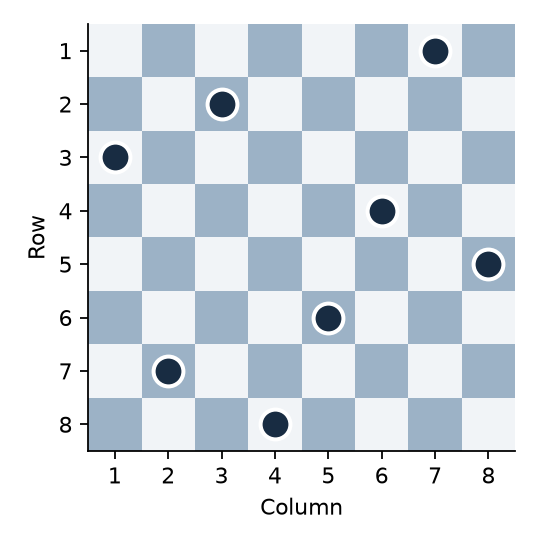
\includegraphics[width=.32\linewidth]{figs/board.png}
\caption{A solution of the $8\times8$ instance returned by the SAT solver
and accepted by the independent checker.}
\label{fig:board}
\end{figure}

\subsection{ILP and CP formulations}
The ILP model uses a binary variable $x_{rc}$ for every square
$(r,c)\in I^2$, with $x_{rc}=1$ if and only if a queen occupies the square.
Let $D_d^-=\{(r,c):r-c=d\}$ and $D_s^+=\{(r,c):r+c=s\}$ denote the
descending and ascending diagonals. The model is
\begin{align}
\sum_{c\in I}x_{rc}&=1 &&\forall r\in I,\label{eq:ilp-row}\\
\sum_{r\in I}x_{rc}&=1 &&\forall c\in I,\label{eq:ilp-col}\\
\sum_{(r,c)\in D_d^-}x_{rc}&\le1 &&\forall d:|D_d^-|\ge2,\label{eq:ilp-down}\\
\sum_{(r,c)\in D_s^+}x_{rc}&\le1 &&\forall s:|D_s^+|\ge2,\label{eq:ilp-up}\\
x_{rc}&\in\{0,1\} &&\forall (r,c)\in I^2,
\end{align}
with a constant objective. For $n\ge2$ the model has $n^2$ variables and
$6n-6$ constraints, because the four single-square diagonals need no
constraint. Gurobi and CPLEX MIP solve the identical model.

The CP model uses the integer variables $q_r\in I$ of the problem
definition and states Constraints~\eqref{eq:column}--\eqref{eq:up} as
three global constraints:
\begin{equation}
\operatorname{AllDifferent}(q_r)_{r\in I},\quad
\operatorname{AllDifferent}(q_r+r)_{r\in I},\quad
\operatorname{AllDifferent}(q_r-r)_{r\in I}.
\end{equation}
CPLEX CP Optimizer and OR-Tools CP-SAT solve the identical model.
No model receives symmetry-breaking constraints, a warm start, or a
precomputed placement.

\subsection{Related work}
\textit{N-queens.} Bell and Stevens~\cite{bell} survey the results on the
problem, including explicit constructions for every $n\ge4$ and its many
variants. Gent et al.~\cite{gent} proved that N-queens completion is
NP-complete and that counting its completions is \#P-complete. The
empty-board problem is therefore studied here as a structured benchmark
for exact solvers rather than as a hard decision problem.

\textit{At-most-one encodings.} Prestwich~\cite{prestwich} reviews CNF
encodings of finite-domain and cardinality constraints. The pairwise
encoding needs no auxiliary variables but a quadratic number of clauses.
The binary encoding of Frisch and Peugniez~\cite{frischbinary} uses a
logarithmic number of auxiliary variables. Sinz~\cite{sinz} introduced
the sequential counter, whose AMO case has linear size and maintains arc
consistency by unit propagation. Klieber and Kwon~\cite{commander}
proposed the commander encoding, which applies AMO hierarchically to
groups of variables, and Chen~\cite{product} proposed the product
encoding, which maps the variables onto a two-dimensional grid. Nguyen
and Mai~\cite{nguyenmai} combined the binary and commander ideas in the
bimander encoding. For sequences of overlapping AMO constraints, Truong
et al.~\cite{staircase} share sequential-counter sub-formulae between
consecutive constraints and reduce both variables and clauses. Comparative
studies~\cite{frischamok} report that no single encoding is best across
problems, which motivates an evaluation on the problem at hand.

\textit{Exact solvers.} Modern SAT solvers follow the conflict-driven
clause learning (CDCL) scheme introduced by GRASP~\cite{grasp}. The SAT
solvers evaluated here are MiniSat~\cite{minisat}, Glucose, which ranks
learned clauses by literal block distance~\cite{glucose},
CaDiCaL~\cite{cadical}, and MapleChrono, which adds chronological
backtracking~\cite{chrono}; all four are accessed through
PySAT~\cite{pysat}. In CP, the all-different constraint has a filtering
algorithm based on bipartite matching~\cite{regin}. CPLEX CP
Optimizer~\cite{cpoptimizer} is a CP engine with automatic search, and
OR-Tools CP-SAT~\cite{cpsat} combines CP propagators with a CDCL SAT core.
Gurobi~\cite{gurobi} and CPLEX~\cite{cplex} solve ILP models by LP-based
branch and cut.

\section{SAT encoding for the N-queens problem}
\label{sec:sat}
\subsection{Encoding overview}
The SAT encoding uses the same occupancy variables $x_{rc}$ as the ILP
model, numbered $rn+c+1$ in DIMACS format. Table~\ref{tab:notation}
summarizes the notation. For a set of literals $X$, let
\begin{equation}
\ALO(X)=\bigvee_{x\in X}x,\qquad
\EO(X)=\ALO(X)\wedge\AMO(X),
\end{equation}
where $\AMO(X)$ is the CNF produced by one of the AMO encodings in
Section~\ref{sec:amo}. Let $R_r$, $C_c$, and $\mathcal D$ denote the
rows, the columns, and the set of diagonals with at least two squares.
We consider two formulations. The \emph{minimal} formulation
\begin{equation}
F_{\min}=\bigwedge_{r\in I}\EO(R_r)\ \wedge\
\bigwedge_{c\in I}\AMO(C_c)\ \wedge\
\bigwedge_{D\in\mathcal D}\AMO(D)
\label{eq:fmin}
\end{equation}
contains only the constraints needed for correctness, and the
\emph{extended} formulation
\begin{equation}
F_{\mathrm{ext}}=F_{\min}\wedge\bigwedge_{c\in I}\ALO(C_c)
\label{eq:fext}
\end{equation}
adds $n$ redundant column clauses and no variables. The redundant
clauses mirror the column equality~\eqref{eq:ilp-col} of the ILP model
and make column occupancy directly available to unit propagation.
\begin{table}[pos=htbp]
\centering\small
\caption{Notation.}
\label{tab:notation}
\begin{tabular}{ll}\toprule
Symbol & Description\\\midrule
$n$ & Board side; the number of queens\\
$I$ & Row and column indices $\{0,\ldots,n-1\}$\\
$x_{rc}$ & Boolean variable: a queen occupies square $(r,c)$\\
$R_r,\ C_c$ & Literals of row $r$ and column $c$\\
$\mathcal D$ & Diagonals with at least two squares ($4n-6$ for $n\ge2$)\\
$\ALO,\ \AMO,\ \EO$ & At-least-one, at-most-one, exactly-one constraints\\
$k$ & Number of inputs of one AMO constraint\\
$a_E(k),\ c_E(k)$ & Auxiliary variables and clauses of encoding $E$ for $k$ inputs\\
$F_{\min},\ F_{\mathrm{ext}}$ & Minimal and extended formulations\\
\bottomrule
\end{tabular}
\end{table}

\begin{proposition}
\label{prop:correct}
For every $n\ge1$ and every correct AMO encoding, the projections of the
models of $F_{\min}$ and of $F_{\mathrm{ext}}$ onto the variables $x_{rc}$
are exactly the feasible placements of Constraints~\eqref{eq:column}--\eqref{eq:up}.
\end{proposition}
The proof is given in Appendix~\ref{app:correct}. The solution is decoded
from the $n^2$ board variables only, so auxiliary variables cannot create
queens.

\subsection{At-most-one encodings}
\label{sec:amo}
Let $X=(x_1,\ldots,x_k)$ be the inputs of one AMO constraint. An encoding
$E(X,Y)$ with auxiliary variables $Y$ is correct if
$\AMO(X)\Leftrightarrow\exists Y\,E(X,Y)$. Fresh auxiliary variables are
created for every AMO constraint, and constraints with $k\le1$ produce no
clauses. The pairwise, commander, and product encodings are implemented
directly; the binary and sequential counter encodings are generated by
PySAT~\cite{pysatcard}.

\textit{Pairwise.} The pairwise encoding forbids every pair of true inputs:
\begin{equation}
E_{\mathrm{pair}}(X)=\bigwedge_{1\le i<j\le k}(\neg x_i\vee\neg x_j).
\end{equation}
It uses no auxiliary variables and $\binom{k}{2}$ clauses.

\textit{Binary.} The binary encoding~\cite{frischbinary} introduces
$b=\lceil\log_2k\rceil$ bits $y_0,\ldots,y_{b-1}$ and assigns input $x_i$
the binary representation of $i-1$. Let $\ell_{it}$ be $y_t$ if bit $t$ of
that representation is one and $\neg y_t$ otherwise. Then
\begin{equation}
E_{\mathrm{bin}}(X,Y)=\bigwedge_{i=1}^{k}\bigwedge_{t=0}^{b-1}(\neg x_i\vee\ell_{it}).
\end{equation}
A true input fixes all bits, which falsifies every other input. The
encoding uses $b$ auxiliary variables and $kb$ clauses for $k\ge3$; PySAT
encodes $k=2$ with one pairwise clause.

\textit{Commander.} The commander encoding~\cite{commander} partitions $X$
into $m=\lceil k/3\rceil$ consecutive groups $G_1,\ldots,G_m$ of at most
three inputs and introduces a commander variable $a_j$ per group:
\begin{equation}
E_{\mathrm{cmd}}(X,A)=\bigwedge_{j=1}^m\Big[E_{\mathrm{pair}}(G_j)\wedge
\bigwedge_{x\in G_j}(\neg x\vee a_j)\wedge
\big(\neg a_j\vee\textstyle\bigvee_{x\in G_j}x\big)\Big]\wedge E_{\mathrm{cmd}}(A).
\end{equation}
The commanders are constrained recursively, and the recursion stops with
the pairwise encoding when $k\le4$. A true input forces its commander,
which excludes the other commanders and hence the inputs of other groups.

\textit{Product.} The product encoding~\cite{product} places the inputs on
a $p\times q$ grid with $p=\lceil\sqrt k\rceil$ and $q=\lceil k/p\rceil$.
Input $x_i$ occupies row $u(i)=\lfloor(i-1)/q\rfloor+1$ and column
$v(i)=((i-1)\bmod q)+1$ of the grid, and
\begin{equation}
E_{\mathrm{prod}}(X,U,V)=\bigwedge_{i=1}^k\big[(\neg x_i\vee u_{u(i)})\wedge
(\neg x_i\vee v_{v(i)})\big]\wedge E_{\mathrm{prod}}(U)\wedge E_{\mathrm{prod}}(V).
\end{equation}
Two distinct inputs differ in a grid row or a grid column and therefore
violate one of the recursive AMO constraints. The recursion stops with
the pairwise encoding when $k\le4$.

\textit{Sequential counter.} The sequential counter~\cite{sinz} introduces
prefix variables $s_1,\ldots,s_{k-1}$, where $s_i$ is true if one of
$x_1,\ldots,x_i$ is true:
\begin{equation}
(\neg x_1\vee s_1)\wedge(\neg x_k\vee\neg s_{k-1})\wedge
\bigwedge_{i=2}^{k-1}\big[(\neg x_i\vee s_i)\wedge(\neg s_{i-1}\vee s_i)
\wedge(\neg x_i\vee\neg s_{i-1})\big].
\end{equation}
It uses $k-1$ auxiliary variables and $3k-4$ clauses for $k\ge3$.

For all five encodings, setting one input to true falsifies all other
inputs of the same constraint by unit propagation alone. Appendix~\ref{app:correct}
describes how this property and the correctness of every encoding were
verified.

\subsection{Encoding size analysis}
Let $a_E(k)$ and $c_E(k)$ be the auxiliary variables and clauses of
encoding $E$ for one constraint with $k\ge2$ inputs. Pairwise gives
$(0,\binom k2)$, binary $(\lceil\log_2k\rceil,k\lceil\log_2k\rceil)$, and
sequential counter $(k-1,3k-4)$, where binary and sequential counter use
$(0,1)$ for $k=2$. For commander and product, $k\le4$ uses the pairwise
counts, and larger constraints follow the recurrences
\begin{align}
a_{\mathrm{cmd}}(k)&=m+a_{\mathrm{cmd}}(m), &
c_{\mathrm{cmd}}(k)&=\textstyle\sum_{j=1}^m\binom{|G_j|}{2}+k+m+c_{\mathrm{cmd}}(m),\\
a_{\mathrm{prod}}(k)&=p+q+a_{\mathrm{prod}}(p)+a_{\mathrm{prod}}(q), &
c_{\mathrm{prod}}(k)&=2k+c_{\mathrm{prod}}(p)+c_{\mathrm{prod}}(q).
\end{align}
For $n\ge2$ the board has $2n+2$ constraints of length $n$ (rows,
columns, and the two main diagonals) and four constraints of each length
$k=2,\ldots,n-1$. The total number of variables and clauses of the
minimal formulation is therefore
\begin{align}
V_E(n)&=n^2+(2n+2)\,a_E(n)+4\sum_{k=2}^{n-1}a_E(k),\label{eq:size-vars}\\
C_{E,\min}(n)&=n+(2n+2)\,c_E(n)+4\sum_{k=2}^{n-1}c_E(k),\label{eq:size-clauses}
\end{align}
where the first term $n$ counts the row ALO clauses. The extended
formulation has the same variables and $C_{E,\min}(n)+n$ clauses. For
the pairwise encoding, Equation~\eqref{eq:size-clauses} evaluates to
$C_{\mathrm{pair},\min}(n)=(5n^3-6n^2+4n)/3$. Table~\ref{tab:amo}
summarizes the asymptotic sizes, and Figure~\ref{fig:sizes} plots the
exact counts. Equations~\eqref{eq:size-vars} and~\eqref{eq:size-clauses}
were checked against the generated CNF for every board size used in the
experiments.
\begin{table}[pos=htbp]
\centering\small
\caption{Asymptotic size of the complete board CNF.}
\label{tab:amo}
\begin{tabular}{lrr}\toprule
Encoding & Auxiliary variables & Clauses\\\midrule
Pairwise & 0 & $\Theta(n^3)$\\
Binary & $\Theta(n\log n)$ & $\Theta(n^2\log n)$\\
Commander & $\Theta(n^2)$ & $\Theta(n^2)$\\
Product & $\Theta(n^{3/2})$ & $\Theta(n^2)$\\
Sequential counter & $\Theta(n^2)$ & $\Theta(n^2)$\\\bottomrule
\end{tabular}
\end{table}
\begin{figure}[pos=htbp]
\centering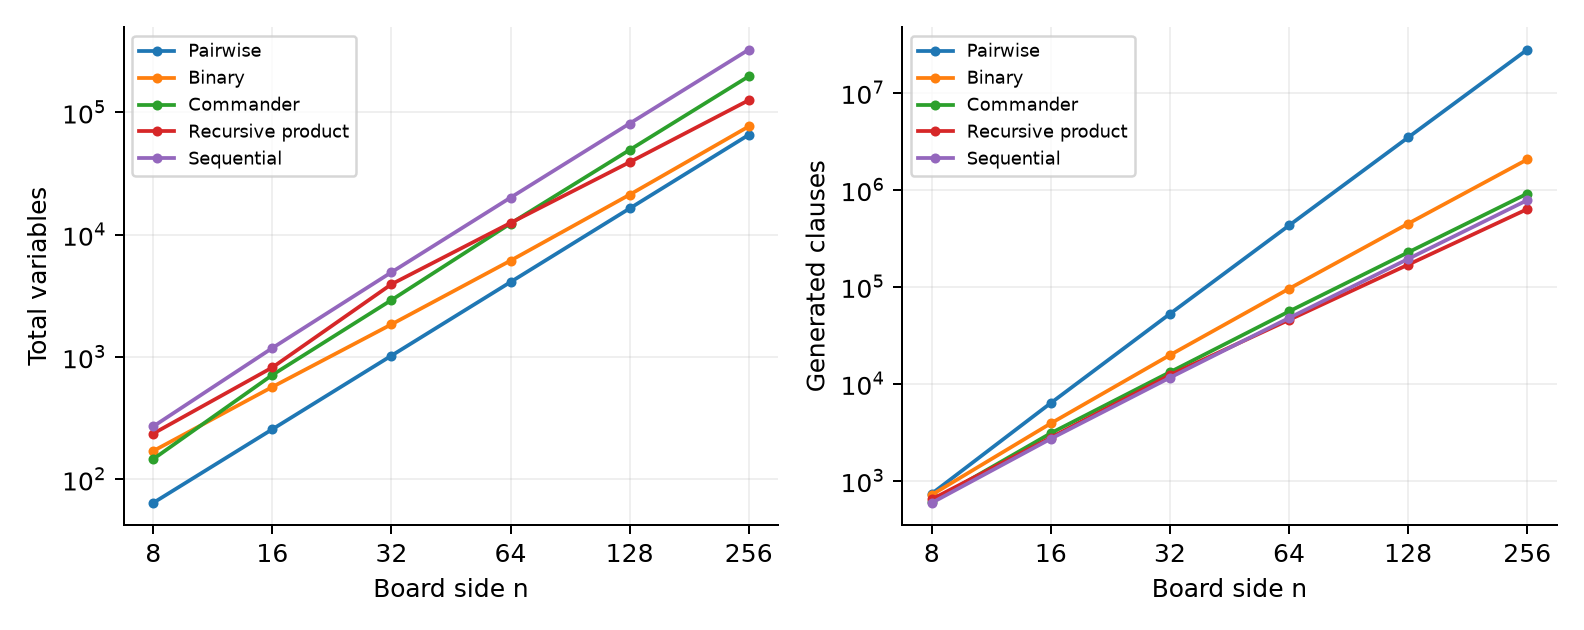
\includegraphics[width=.92\linewidth]{figs/formula_sizes.png}
\caption{Total variables (left) and clauses (right) of the minimal
formulation as a function of the board side $n$, on logarithmic axes.}
\label{fig:sizes}
\end{figure}
\FloatBarrier
For $n=\res{encodings/maxn}$ the pairwise encoding generates
\res{size/pairwise/256/clauses} clauses, whereas the commander, product, and
sequential counter encodings generate \res{size/commander/256/clauses},
\res{size/product/256/clauses}, and \res{size/seqcounter/256/clauses}
clauses. The binary encoding uses the fewest variables
(\res{size/binary/256/vars}) but more clauses
(\res{size/binary/256/clauses}) than the other non-pairwise encodings.

\section{Experimental setup}
\label{sec:setup}
\subsection{Implementation}
The SAT encoder, the CP and ILP models, and the experiment harness are
written in Python. The encoder streams clauses directly into the SAT
solver and can also export the formula in DIMACS format. The CP model is
passed to CPLEX CP Optimizer through DOcplex~\cite{ibm} and to CP-SAT
through the OR-Tools Python interface; the ILP model is passed to Gurobi
and CPLEX through their Python interfaces. Every returned placement is
checked by an independent validator for its length, domain, and
uniqueness of columns and of both diagonal indices.

\subsection{Benchmark instances and experiments}
The benchmark consists of the empty $n\times n$ boards listed in
Table~\ref{tab:experiments}. Three experiments are performed.
Experiment~E1 compares the ten combinations of five AMO encodings and two
formulations using CaDiCaL. Experiment~E2 fixes the best configuration of
E1 and compares four SAT solvers. Experiment~E3 compares the resulting SAT
configuration with CPLEX CP, CPLEX MIP, Gurobi, and CP-SAT and extends
the board side to $n=\res{exact/maxn}$.
\begin{table}[pos=htbp]
\centering\small
\caption{Summary of the experiments. Each configuration is run once on each board.}
\label{tab:experiments}
\begin{tabular}{llll}\toprule
Experiment & Board sides $n$ & Methods & Runs\\\midrule
E1: AMO encodings & 8, 16, 32, 64, 128, 256 & 5 encodings $\times$ 2 formulations, CaDiCaL & 60\\
E2: SAT solvers & 8, 16, 32, 64, 128, 256 & CaDiCaL, Glucose, MiniSat, MapleChrono & 24\\
E3: exact solvers & 8, 16, \ldots, 256, 512, 1024 & SAT, CPLEX CP, CPLEX MIP, Gurobi, CP-SAT & 40\\
\bottomrule
\end{tabular}
\end{table}

\subsection{Environment and metrics}
All experiments were conducted on a laptop with an AMD Ryzen 7 8845HS
processor (8 cores, 16 threads) and 32 GB of RAM, running Windows 11 Home.
We used Python 3.14, PySAT 1.9.dev2 with CaDiCaL 1.9.5, Glucose 4.2,
MiniSat 2.2, and MapleChrono, Gurobi 13.0.3, IBM ILOG CPLEX Optimization
Studio 22.2 (CPLEX MIP and CP Optimizer), and OR-Tools 9.15. Every solver
uses one thread and random seed 1. Each run is executed in a fresh process with a time
limit of \res{budget}~s, which covers library imports, license
acquisition, model construction, and solving. A run that exceeds the
limit is recorded as a timeout (TO). The experiments were run
sequentially, one solver process at a time.

We report three metrics. \emph{Process time} is the wall-clock time of the
complete run and is the primary metric. \emph{Core time} is the time for
model construction and solving only, which excludes imports and license
acquisition. \emph{PAR-2} is the mean process time over all runs of a
method, where each timeout counts as twice the time limit
(\res{par2penalty}~s). Because each configuration is run once, tables report that single
measurement and TO marks a timeout. The laptop was shared with other jobs,
so absolute times carry noise and only large differences should be read as
real.

\section{Experimental results}
\label{sec:results}
\subsection{AMO encodings}
Table~\ref{tab:enc} ranks the ten configurations of Experiment~E1 by PAR-2.
The commander encoding with the minimal formulation is best
(\res{encodings/cadical195-commander-minimal/par2}~s), followed by the
commander encoding with the extended formulation
(\res{encodings/cadical195-commander-extended/par2}~s). The pairwise
encoding timed out at $n=\res{encodings/maxn}$ because its formula has
\res{size/pairwise/256/clauses} clauses. The product and sequential counter
encodings in the minimal formulation also timed out at that size, while their
extended variants solved it in \res{encodings/cadical195-product-extended/256/time}~s
and \res{encodings/cadical195-seqcounter-extended/256/time}~s. The redundant column
ALO clauses of the extended formulation therefore helped the product,
sequential counter, and binary encodings, but did not help the commander
encoding, whose minimal formulation was faster
(\res{encodings/cadical195-commander-minimal/256/time}~s against
\res{encodings/cadical195-commander-extended/256/time}~s). Figure~\ref{fig:enc}
shows the PAR-2 time as a function of $n$.
\begin{table}[pos=htbp]
\centering\small
\caption{Experiment E1: encodings ranked by PAR-2 over six board sizes with CaDiCaL.}
\label{tab:enc}\begin{tabular}{lrrrr}
\toprule
Encoding / formulation & Solved & PAR-2 (s) & Variables & Clauses \\
\midrule
commander/minimal & 18/18 & 0.450 & 49,354 & 226,242 \\
commander/extended & 18/18 & 0.459 & 49,354 & 226,370 \\
product/extended & 18/18 & 0.921 & 39,174 & 169,112 \\
binary/extended & 18/18 & 1.221 & 21,234 & 447,828 \\
seqcounter/extended & 18/18 & 1.275 & 81,150 & 193,800 \\
pairwise/minimal & 18/18 & 1.863 & 16,384 & 3,462,656 \\
pairwise/extended & 18/18 & 1.898 & 16,384 & 3,462,784 \\
binary/minimal & 18/18 & 3.113 & 21,234 & 447,700 \\
seqcounter/minimal & 15/18 & 5.718 & 81,150 & 193,672 \\
product/minimal & 12/18 & 7.534 & 39,174 & 168,984 \\
\bottomrule
\end{tabular}

\end{table}
\begin{figure}[pos=htbp]
\centering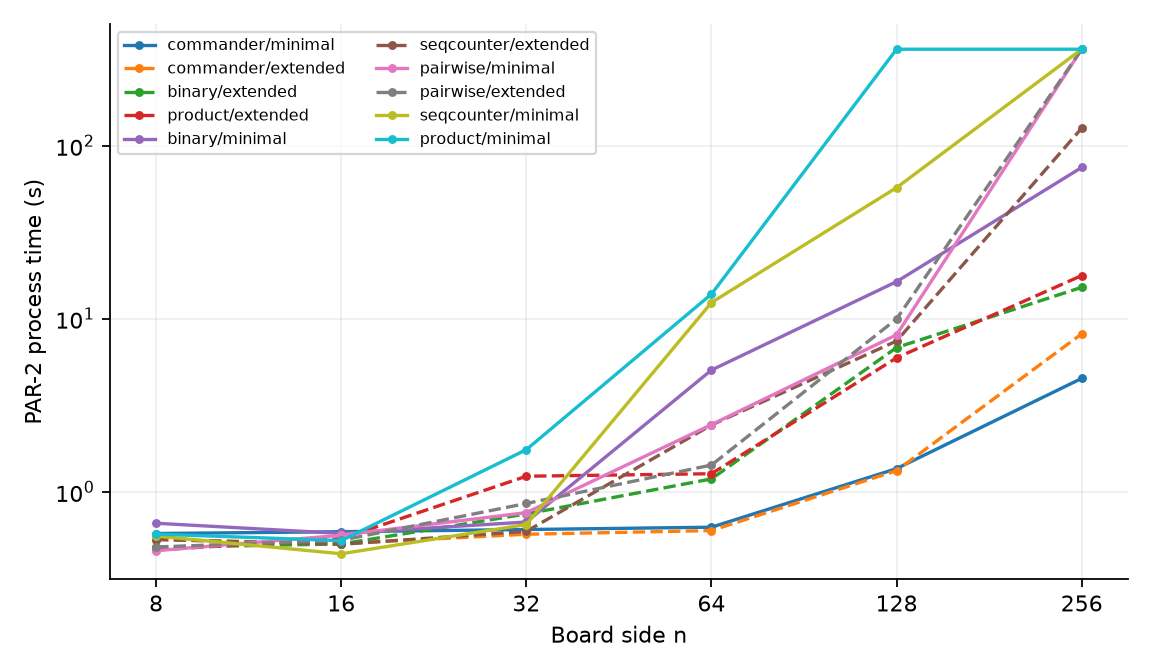
\includegraphics[width=.8\linewidth]{figs/encodings.png}
\caption{PAR-2 process time of the ten SAT configurations.}
\label{fig:enc}
\end{figure}

\subsection{SAT solvers}
Table~\ref{tab:solvers} compares the solvers on the commander encoding with
the minimal formulation. CaDiCaL solved all boards
(PAR-2 \res{solvers/cadical195-commander-minimal/par2}~s) and MiniSat solved
all of them but was slower at large $n$. Glucose
(\res{solvers/glucose42-commander-minimal/solved} solved) and MapleChrono
(\res{solvers/maplechrono-commander-minimal/solved} solved) timed out on the larger
boards.
\begin{table}[pos=htbp]
\centering\small
\caption{Experiment E2: process time (s) of four SAT solvers.}
\label{tab:solvers}\begin{tabular}{lrrrr}
\toprule
$n$ & CaDiCaL & Glucose & MiniSat & MapleChrono \\
\midrule
8 & 0.82 & 1.32 & 0.81 & 0.81 \\
16 & 0.77 & 0.69 & 0.75 & 24.00 \\
32 & 0.99 & 48.00 & 0.65 & 31.07 \\
64 & 0.86 & 20.21 & 0.81 & TO \\
128 & 2.24 & TO & 13.95 & TO \\
256 & 11.76 & TO & 13.42 & TO \\
Solved & 6/6 & 4/6 & 6/6 & 3/6 \\
PAR-2 & 2.91 & 131.7 & 5.07 & 189.3 \\
\bottomrule
\end{tabular}

\end{table}

\subsection{Comparison with CP and ILP solvers}
Table~\ref{tab:exact} and Figure~\ref{fig:exact} compare the SAT
configuration with the CP and ILP solvers. Up to $n=64$ all methods finish
within a few seconds, and the differences come mostly from start-up cost.
From $n=128$ the solvers separate. CPLEX CP and Gurobi solved every board,
including $n=\res{exact/maxn}$ in \res{scaling/cplex-cp/1024/time}~s and
\res{scaling/gurobi/1024/time}~s. The SAT configuration needed
\res{scaling/cadical195-commander-minimal/512/time}~s at $n=512$ and timed
out at $n=\res{exact/maxn}$, as did CPLEX MIP. CP-SAT was the slowest, taking
\res{exact/cpsat/256/time}~s at $n=256$ and timing out beyond it.
\begin{table}[pos=htbp]
\centering\small
\caption{Experiment E3: process time (s) of the SAT configuration and the CP and ILP solvers.}
\label{tab:exact}\begin{tabular}{lrrrrr}
\toprule
$n$ & SAT & CPLEX CP & CPLEX MIP & Gurobi & CP-SAT \\
\midrule
8 & 0.247 & 1.510 & 0.401 & 0.345 & 1.325 \\
16 & 0.264 & 1.496 & 0.427 & 0.357 & 1.354 \\
32 & 0.272 & 1.443 & 0.427 & 0.344 & 1.370 \\
64 & 0.363 & 1.466 & 0.467 & 0.423 & 1.725 \\
96 & 0.685 & 1.462 & 0.517 & 0.412 & 2.529 \\
128 & 0.871 & 1.503 & 0.606 & 0.700 & 3.838 \\
256 & 4.085 & 1.419 & 1.248 & 0.854 & TO (0/3) \\
512 & TO (0/3) & 1.440 & 5.617 & 2.367 & TO (0/3) \\
\bottomrule
\end{tabular}

\end{table}
\begin{figure}[pos=htbp]
\centering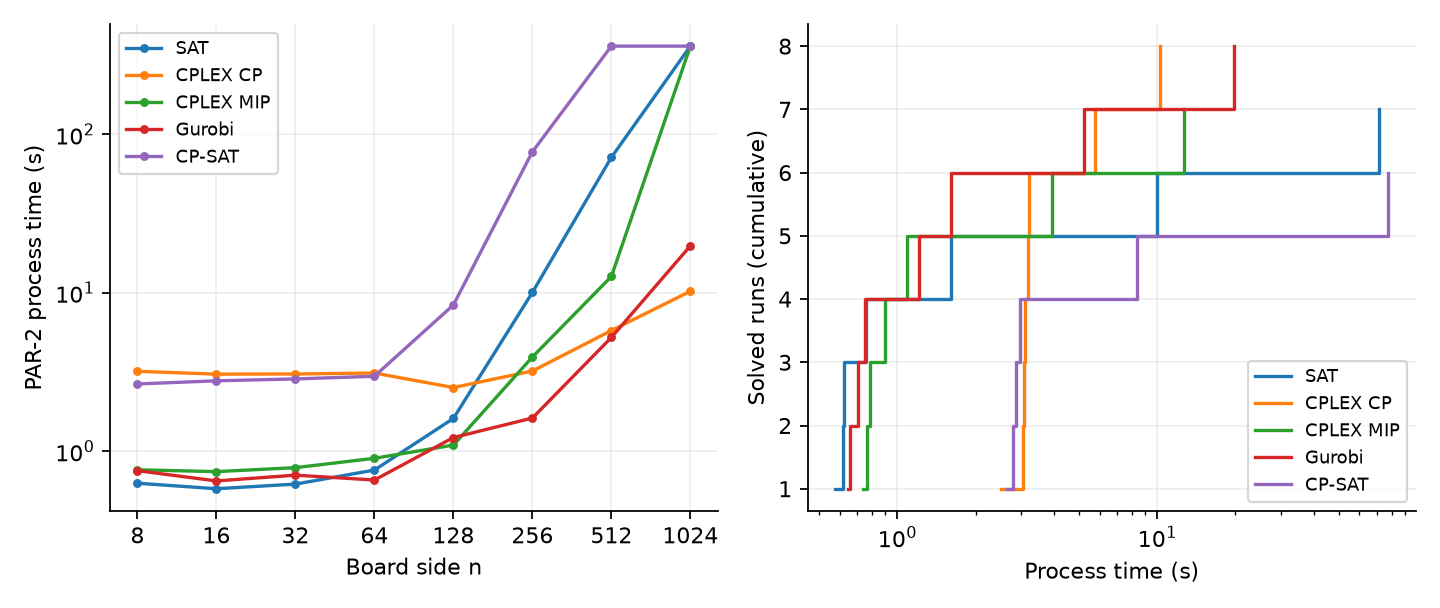
\includegraphics[width=\linewidth]{figs/exact.png}
\caption{PAR-2 time against board side (left) and cumulative solved runs (right).}
\label{fig:exact}
\end{figure}
\FloatBarrier

\subsection{Discussion}
The choice of AMO encoding matters more than the choice between the two
formulations: the gap between the best and worst encodings at
$n=\res{encodings/maxn}$ is a timeout against a few seconds, and the
encodings that add auxiliary variables hierarchically (commander, product)
keep the clause count near $\Theta(n^2)$ while the pairwise encoding grows
as $\Theta(n^3)$. On this problem a dedicated CP propagator or an LP-based
solver still beats the best SAT model on very large boards, because the SAT
formula grows quadratically. Threats to validity are the single run per
configuration, the shared machine, and the 180~s limit, which turns slow
runs into censored observations.

\section{Conclusion}
\label{sec:conclusion}
We compared five AMO encodings, two formulations, four SAT solvers, and four
CP and ILP solvers on the N-queens problem. The commander encoding with the
minimal formulation and CaDiCaL was the best SAT configuration, and the extended
formulation helped all encodings except commander. CPLEX CP and Gurobi were the
only methods to solve every board up to $n=\res{exact/maxn}$. The results come
from one run per configuration on a shared laptop, so they show broad trends
rather than precise rankings. A natural extension is repeated runs on a
dedicated machine.

\section*{CRediT authorship contribution statement}
\textbf{Do Duc Long:} Conceptualization, Methodology, Software,
Validation, Investigation, Data curation, Visualization,
Writing -- original draft, Writing -- review \& editing.

\section*{Declaration of competing interest}
The author declares no known competing financial interests or personal
relationships that could have appeared to influence the work
reported in this paper.

\section*{Data availability}
The source code, raw results, returned placements, and report sources are
available at \url{https://github.com/dolong226/homework1-nqueens}.

\appendix
\section{Correctness of the SAT encoding}
\label{app:correct}
\textit{Proof of Proposition~\ref{prop:correct}.} Let $\sigma$ be a model of
$F_{\min}$. The row constraints $\EO(R_r)$ place exactly one queen in each
row, so $\sigma$ defines a vector $q$ with $q_r$ equal to the column of the
queen in row $r$. The column constraints $\AMO(C_c)$ forbid two of these
$n$ queens in one column, which gives Constraint~\eqref{eq:column}, and the
diagonal constraints give Constraints~\eqref{eq:down} and~\eqref{eq:up}.
Conversely, a feasible placement satisfies every ALO and AMO constraint
on the board variables, and each correct AMO encoding can extend it to
its auxiliary variables. The same placement also satisfies the column ALO
clauses of $F_{\mathrm{ext}}$, because $n$ queens in $n$ distinct columns
occupy every column. Hence both formulations have the same projected
models. \hfill$\square$

\textit{Correctness of the AMO encodings.} Each encoding is correct for
the following reasons. In the pairwise encoding, two true inputs violate
their clause. In the binary encoding, two true inputs require different
bit patterns. In the commander encoding, two true inputs in one group
violate a pairwise clause, and two true inputs in different groups force
two commanders. In the product encoding, two true inputs force two grid
rows or two grid columns. In the sequential counter, a true input $x_i$
forces $s_i,s_{i+1},\ldots$ and thereby falsifies every later input.
Conversely, an assignment with at most one true input is extended by
setting each auxiliary variable to the disjunction of the inputs it
represents, and the all-false assignment is extended by setting all
auxiliary variables to false.

\textit{Automated verification.} The implementation was verified by three
test suites. First, every truth assignment of every AMO encoding was
enumerated for $k=0,\ldots,11$ inputs with positive and negative literals.
Second, all solutions of the ten SAT configurations were enumerated for
$n=1,\ldots,8$ with blocking clauses over the board variables only and
compared with an independent backtracking solver; the counts
$1,0,0,2,10,4,40,92$ match. Third, for $k=1,\ldots,64$, setting each input
to true was shown to falsify all other inputs by unit propagation alone.
The CP and ILP models were checked on the infeasible board $n=3$ and the
feasible board $n=8$.

\section{Detailed encoding results}
\label{app:sizes}
\begin{table}[pos=htbp]
\centering\small
\caption{Median process time (s) of each encoding and formulation with
CaDiCaL on each board size (Experiment~E1).}
\label{tab:enc-sizes}\begin{tabular}{lrrrrrr}
\toprule
Encoding / formulation & $n=8$ & $n=16$ & $n=32$ & $n=64$ & $n=96$ & $n=128$ \\
\midrule
pairwise/minimal & 0.253 & 0.271 & 0.355 & 1.262 & 3.141 & 5.795 \\
binary/minimal & 0.263 & 0.286 & 0.413 & 2.667 & 8.791 & 6.218 \\
commander/minimal & 0.253 & 0.261 & 0.282 & 0.382 & 0.609 & 0.886 \\
product/minimal & 0.254 & 0.285 & 0.708 & 3.738 & TO (0/3) & TO (0/3) \\
seqcounter/minimal & 0.260 & 0.265 & 0.348 & 4.294 & 8.936 & TO (0/3) \\
pairwise/extended & 0.268 & 0.272 & 0.484 & 0.987 & 2.516 & 6.769 \\
binary/extended & 0.259 & 0.289 & 0.405 & 0.751 & 2.217 & 3.362 \\
commander/extended & 0.263 & 0.262 & 0.276 & 0.376 & 0.666 & 0.888 \\
product/extended & 0.266 & 0.269 & 0.481 & 0.648 & 1.105 & 2.736 \\
seqcounter/extended & 0.252 & 0.278 & 0.355 & 1.250 & 2.128 & 3.331 \\
\bottomrule
\end{tabular}

\end{table}
\FloatBarrier

\section*{Declaration of generative AI and AI-assisted technologies}
During the preparation of this work the author used OpenAI Codex and
Claude Code (Anthropic) to assist with implementation, experiment
automation, and editing of the manuscript. After using these tools, the
author reviewed and edited the content as needed and takes full
responsibility for the content of the publication.

\bibliographystyle{cas-model2-names}
\bibliography{refs}
\end{document}
